\documentclass[a4paper,english,titlepage,11pt]{article}

\usepackage{mathcomp,amssymb,mathptm,verimagstudent}
\usepackage[utf8]{inputenc}
\usepackage[T1]{fontenc}
\usepackage{amsmath}
\usepackage{mathenv}
\usepackage{tikz}
\usepackage{listings}
\usepackage{placeins}

\newtheorem{definition}{Definition}[section]
\newtheorem{theorem}{Theorem}[section]
\newtheorem{proposition}[theorem]{Proposition}


\def\R{\mathbb{R}}
\def\N{\mathbb{N}}
\def\Q{\mathbb{Q}}
\def\P{\mathcal{P}}

\definecolor{trefle}{rgb}{0,0.5,0}
\definecolor{moka}{rgb}{0.5,0.25,0}
\definecolor{minuit}{rgb}{0,0,0.5}

\tikzstyle{arrow}=[->,line width=.05cm,draw=red!90!blue!60!black]

\usetikzlibrary{snakes,arrows,shapes,backgrounds,shadows,automata,patterns}
\usepgflibrary{snakes}

\tikzstyle{state}=[circle,fill=black!25,minimum size=13pt,inner sep=0pt]
\tikzstyle{transition}=[rectangle,thick,draw=black!75,
  			  fill=black!20,minimum size=4mm]
\tikzstyle{transition2}=[rectangle,thick,draw=blue!75,
  			  fill=blue,minimum size=4mm,blue]
\tikzstyle{PRstate}=[circle,fill=red!90,minimum size=13pt,inner sep=0pt]
\tikzstyle{polyhedra}=[blue!25,opacity=0.5,pattern=north west lines,pattern
color=blue]
\tikzstyle{line}=[black,thick]

\lstnewenvironment{C}
{\lstset{language=C,
		basicstyle=\ttfamily,
		commentstyle=\color{moka}\textit,
		keywordstyle=\color{minuit},
		identifierstyle=\color{trefle},
		showstringspaces=false}}
{}

\title{Static Analysis by Path Focusing}
\author{Julien Henry}
\date{2011}
\shorttitle{Static Analysis by Path Focusing}
\institute{Grenoble-INP}
\abstract{an abstract}
\keywords{keywords}
\tutor{David Monniaux - Matthieu Moy}
\notes{some notes}
\webaddress{Julien.Henry@imag.fr}
\reporttype{M2R internship's report}


\begin{document}
  
  \maketitlepage

  \tableofcontents
  
  \newpage


\section*{Introduction} 

\part{Abstract Interpretation: state of the art}

\section{Abstract Interpretation}

Abstract Interpretation \cite{CC77,CousotCousot92-1} is a general method to find approximate solutions of
fixpoint equations. This method is used for program analysis, since analyzing a
program often comes down to solving fixpoint equations $\Phi(x) = x$.

However, most of the time, the solution of this fixpoint equation must be
computed in a complex domain: in program analysis, this could be the state space
of the program, i.e the set of all possible states of the program. This
computation quickly becomes too costly.

\subsection{Abstraction of the domain}

Abstract Interpretation method proposes to represent more efficiently the
elements of this complex domain $C$ of concrete values, by choosing an simpler
domain  $A$ called \emph{abstract domain}. The relation between these two
domains is characterized by two functions, usually called 
$\alpha\ :\ C \mapsto A$, $\gamma \ : \ A \mapsto C$, such as:

$$\forall x \in C, \forall y \in A, \alpha(x) \leq_{A} y \Leftrightarrow x
\leq_{C} \gamma(y) $$

where $\leq_C$ and $\leq_A$ are the order relations on $C$ and $A$. Then, the
fixpoint computation is done in the abstract domain, using the approximation of
the function $\Phi$, i.e $\alpha(\Phi) = \alpha \circ \Phi \circ \gamma$, also
noted $\Phi^\#$.
We have the following result:

\begin{proposition}
If $C$ is a complete lattice, and if $\Phi$ is increasing from $C$ to $C$, then
$$\alpha(lfp(\Phi)) \leq_A lfp(\alpha(\Phi))$$
where $lfp(\Phi)$ denotes the least fixpoint of $\Phi$.
\end{proposition}

In fact, one compute the least fixpoint of the function in the abstract
domain, and the result of the computation also gives an upper approximation of
the fixpoint in the concrete domain.


\subsection{Termination}

Termination of the fixpoint computation has to be guaranteed. This termination
depends on the properties of the abstract domain:
this one should be finite, or of finite depth, meaning that there doesn't exist
any sequence $(y_i)_{i \geq 0}$ of elements of the abstract domain $A$ such as
$\forall i \geq 0,\ y_i \leq_A y_{i+1}$. Indeed, in case of a domain of infinite
depth, the least fixpoint
computation could run indefinitely, since the ascending sequence of elements of
$A$ is infinite, and the fixpoint in never reached.


Most of the domains that are used for program analysis doesn't satisfy this
finiteness property. To ensure convergence in this case, another approximation
is performed: a new operator is defined, called \emph{widening operator}, that
extrapolates the limit of a sequence of abstract values
\cite{CC77,CousotCousot92-4}. This \emph{widening
operator} is usually noted $\nabla: A \times A \rightarrow A$, and satisfies
the following properties:

\begin{itemize}
\item $\forall y_1, y_2 \in A,\ y_1 \leq_A y_1 \nabla y_2$ and $y_2 \leq_A y_1
\nabla y_2$. This guarantees the correctness of the result.
\item For any increasing sequence $y_0 \leq_A y_1 \leq_A \dots$, the sequence
defined by 
$$\left\{ \begin{array}{rll}
y'_0 & = &  y_0 \\
y'_{i+1} & = &  y'_i\ \nabla\ y_{i+1},\ \  \forall i > 0
\end{array} \right.$$
is not strictly increasing. Then, applying the widening operator when the
sequence may increase indefinitely makes the computation converge to a fixpoint
in finite time. 
\end{itemize}

The least fixpoint of a function $\Phi^\#$ is noted $\overline{y}$ and is equal
to $\displaystyle \lim_{i \geq 0}\ y_i$, where $y_0 = \perp$ (the least element
of $A$) and $y_{i+1} = \Phi^\# (y_i)$. Instead of computing this least fixpoint,
one compute an upper approximation of it, by computing the following ascending
sequence:

$$\left\{ \begin{array}{rll}
y'_0 &=& \perp \\
y'_{i+1} &=& y'_i\ \nabla\ \Phi^\#(y'_i),\ \ \forall i > 0
\end{array} \right.$$

which converges towards $\tilde{y}$, where $\tilde{y} \geq_A \overline{y}$.

$\tilde{y}$ is a correct upper approximation of the least fixpoint of $\Phi^\#$,
and the classical technique is to regain some precision lost by the widening
operator by computing a descending sequence:

$$\left\{ \begin{array}{rll}
y''_0 &=& \tilde{y} \\
y''_{i+1} &=& \Phi^\#(y''_i), \ \ \forall i > 0
\end{array} \right.$$

Each element of this descending sequence is still an upper approximation of the
least fixpoint $\overline{y}$. So, this sequence often allows to find
approximate least fixpoints that are more precise than the one obtained after
the ascending sequence.

\section{Linear Relation Analysis}

Linear Relation Analysis \cite{CH78} (also noted LRA) is a direct application of
Abstract Interpretation. It aims at computing an upper approximation of the
reachable states of a program containing numerical variables. The set of
possible assignments for the numerical variables is abstracted by convex
polyhedron. This technique discovers invariant linear relations between
the numerical variables at each control point of a program.

\subsection{Convex polyhedra}

Let $x_1, x_2, \dots ,x_n$ be the numerical variables of a program (assume they
all are in $\Q$). A state of
the program is then a point $\overrightarrow{x} \in \Q^n$.

In $\Q^n$, the set of polyhedra is a lattice. The least element is $\perp$
(the empty polyhedron), and the greatest element is $\top$ (the whole $Q^n$).

The classical union of two convex polyhedra may not be a convex polyhedra.
Therefore, we use the convex hull operation, noted $\sqcup$, for joining
polyhedra. 
If $X_1, X_2$ are two convex polyhedra, $X_1 \sqcup X_2$ is the
smallest convex polyhedron containing both $X_1$ and $X_2$.

Since the domain of convex polyhedra is of infinite depth, a widening operator
is defined to ensure convergence of the technique. There have been different
work proposing a definition of the widening operator in LRA
\cite{CH78,Hal79,HPR97,BlanchetCousotEtAl_PLDI03}, in order to fight
against the loss of precision induced by widening.

\subsection{Program Analysis}

Throughout the report, a program will be represented by a control flow graph:
\begin{itemize}
\item $P$ is a finite set of control points.
\item $I_p$ is the (possibly empty)
set of initial values for each control point $p \in P$.
\item $E \subseteq  P \times P$ is a set of directed edges. Each edge $e \in E$
has a semantic $\tau_e: \P(\Q^n) \rightarrow \P(\Q^n)$, $\P(\Q^n)$ being the set
of possible values of $\overrightarrow{x}$. $\tau_e$ maps a set of states before
the transition to the set of states after the transition.
\end{itemize}

\begin{figure}[!h]
   \begin{minipage}[c]{.46\linewidth}
\begin{C}
x = 0;
y = 0;
while (true) {
	if (x <= 50) 
		y++;
	else 
		y--;
	if (y < 0) break;
	x++;
}
\end{C}
   \end{minipage} \hfill
   \begin{minipage}[c]{.46\linewidth}
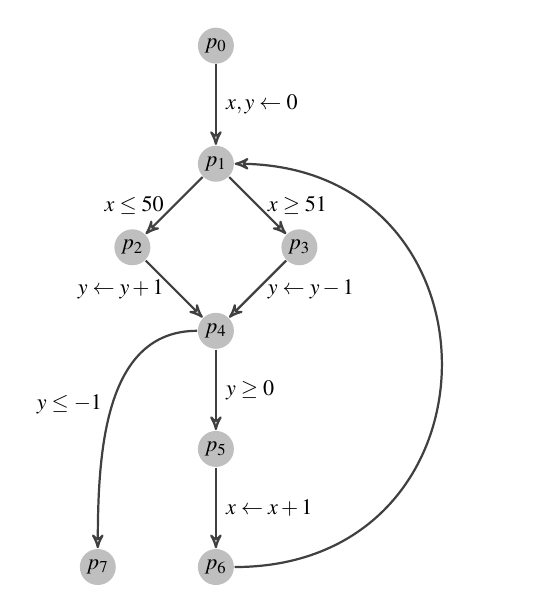
\begin{tikzpicture}[->,>=stealth',auto,node distance=1.5cm,
                    semithick,font=\footnotesize]

	\node[state] (n0) {$p_0$};
	\node[state] (n1) [below of=n0] {$p_1$};
	\node[state] (n2) [below left of=n1] {$p_2$};
	\node[state] (n3) [below right of=n1] {$p_3$};
	\node[state] (n4) [below left of=n3] {$p_4$};
	\node[state] (n5) [below of=n4] {$p_5$};
	\node[state] (n6) [below of=n5] {$p_6$};
	\node[state] (n7) [left of=n6] {$p_7$};

	\node (n8) [right of=n6] {};
	\node (n9) [right of=n1] {};

  \path [transition] 
		(n0) edge              node {$x,y \leftarrow 0$} (n1);
  \path [transition] 
        (n1) edge			   node [left] {$x \leq 50$} (n2);
  \path [transition] 
        (n1)  edge              node [right] {$x \geq 51$} (n3);
  \path [transition] 
        (n2) edge              node [left] {$y \leftarrow y+1$} (n4);
  \path [transition] 
        (n3) edge			   node [right] {$y \leftarrow y-1$} (n4);
  \path [transition] 
        (n4) edge			   node {$y \geq 0$} (n5);
  \path [transition] 
		(n4) edge  [out = 180, in=90] node [left] {$y \leq -1$} (n7);
  \path [transition] 
        (n5) edge              node {$x \leftarrow x+1$} (n6);
  \path [transition] 
        (n6) edge [out=0, in=0, distance=3.5cm] node {} (n1);

\end{tikzpicture}
   \end{minipage}
   \caption{Example of program, and its associate control flow graph. This
   program comes from \cite{GopanR06}.}
\end{figure}
\FloatBarrier

To each state $p \in P$ of the control flow graph, we associate an abstract
value $X_p \in D$, $D$ being in our case the domain of convex polyhedra over
$\Q^n$. Since the exact operation $\tau$ may not be expressed in the abstract
domain, we abstract it into $\tau^\#$ such as $\forall X \in D, \tau(X)
\subseteq \tau^\#(X)$. 

The computation aims to find a solution for this system of abstract semantic
inequalities:

$$\left\{ \begin{array}{l}
\forall p \in P, \ \ I_p \subseteq X_p \\
\forall (p',p) \in E,\ \  \tau^\#_{(p',p)}(X_{p'}) \subseteq X_p
\end{array} \right.$$


The function $\Phi^\#$ previously described is the following:

$$\Phi^\#\left[ \begin{array}{c}
\vdots \\
X_p \\
\vdots
\end{array} \right] = \left[ \begin{array}{c} 
\vdots \\
I_p \sqcup \displaystyle \bigsqcup_{(p',p) \in E} \tau^\# (X_{p'}) \\
\vdots
\end{array} \right]$$

The fixpoint computation algorithm consist in replacing iteratively each $X_p$ by its value
on the right hand side, until the convergence.

In the case of abstract domain with infinite ascending sequence, we use the
previously defined widening operator:

$$\left[ \begin{array}{c}
\vdots \\
X_p \\
\vdots
\end{array} \right] \longleftarrow \left[ \begin{array}{c} 
\vdots \\
X_p \nabla \left( I_p \sqcup \displaystyle \bigsqcup_{(p',p) \in E} \tau^\#
(X_{p'}) \right) \\
\vdots
\end{array} \right]$$



After a finite number of steps, the computation has reached the fixpoint and the
value $X_p$ at the end give the different linear relations between the
different numerical variables of the program at the control point $p$.

\subsection{Precision of the analysis}

In order to guarantee the termination of the computation, there is no need to
apply the widening operator at each control point $p \in P$. It is sufficient to
apply it on a subset of $P$, called $P_w$, such as removing the nodes of $P_w$
disconnect every cycles. For instance, one could choose $P_w$ as the set of the
heads of loops.


There exist several iteration strategies for computing the fixpoint: whatever
the order we choose for updating the different $X_p, p\in P$, the result at the
end of the analysis is correct. Yet, the precision of the result and the time
before convergence could be very different. 
There have been some work to find efficient iteration strategies
\cite{Bou92}, such as first stabilizing innermost loops, or stabilizing strongly
connected components of the graph.

\part{Path Focusing technique}
  
	Pour calculer les variables live en SSA, des algorithmes plus optimisés sont
	expliqués dans la thèse de B. Boissinot\cite{Boi10}

	
	Utilisation de la bibliothèque APRON \cite{JM09}
  

\part{Contribution}

  \section{Conclusion}
  
  \appendix
  

\bibliographystyle{plain}
  \bibliography{report}
\end{document}
